% 建议使用 XeLaTeX 或 LuaLaTeX 编译(中文与公式支持更佳)
\documentclass[UTF8,zihao=-4]{ctexart}

\usepackage[a4paper,margin=2.5cm]{geometry}
\usepackage{amsmath, amssymb, amsthm}
\usepackage{bm}
\usepackage{hyperref}
\usepackage{graphicx}
\usepackage{caption}
\usepackage{listings}
\usepackage{xcolor}
\usepackage{float}
\usepackage{placeins}
\graphicspath{{figures/}}

\lstdefinestyle{code}{
  basicstyle=\ttfamily\small,
  numbers=left,
  numberstyle=\tiny,
  numbersep=8pt,
  keywordstyle=\color{blue},
  commentstyle=\color{teal!70!black},
  stringstyle=\color{orange!70!black},
  showstringspaces=false,
  breaklines=true,
  frame=single,
  framerule=0.3pt,
  rulecolor=\color{black!15}
}
\lstset{style=code}

\title{SARSA 值迭代方法:原理、公式、应用与实战}
\author{}
\date{\today}

\begin{document}
\maketitle

\section{引言}
SARSA(State-Action-Reward-State-Action)是典型的在线策略(on-policy)时间差分强化学习算法。与 Q-learning 的“乐观”最大化不同,SARSA 使用策略实际执行的下一动作更新价值函数,因此能够更好地反映探索策略下的期望表现。

\section{原理与公式}
\subsection{在线策略动作价值函数}
SARSA 估计当前策略 \(\pi\) 下的动作价值函数 \(Q(s,a)\),其贝尔曼方程为:
\begin{equation}
Q^{\pi}(s,a) = \mathbb{E}\big[ r_{t+1} + \gamma Q^{\pi}(s_{t+1}, a_{t+1}) \mid s_t = s, a_t = a \big],
\end{equation}
其中 \(a_{t+1} \sim \pi(\cdot \mid s_{t+1})\)。

\subsection{更新规则}
完成一次交互 \((s_t, a_t, r_{t+1}, s_{t+1}, a_{t+1})\) 后,SARSA 更新为:
\begin{equation}
Q_{t+1}(s_t, a_t) \leftarrow Q_t(s_t, a_t) + \alpha_t \Big[ r_{t+1} + \gamma Q_t(s_{t+1}, a_{t+1}) - Q_t(s_t, a_t) \Big].
\end{equation}
通常采用 \(\varepsilon\)-贪心策略选择动作,上式中的 \(a_{t+1}\) 即为该策略在下一状态给出的动作。

\subsection{收敛性质}
只要学习率满足 \(\sum_t \alpha_t = \infty\)、\(\sum_t \alpha_t^2 < \infty\),且策略确保所有状态-动作对被无限次访问,在有限 MDP 中 SARSA 可收敛到最优 \(\varepsilon\)-贪心策略。由于更新考虑了探索动作,SARSA 在存在危险区域时通常比 Q-learning 更保守。

\section{应用与技巧}
\begin{itemize}
  \item \textbf{随机控制}:如“悬崖行走”环境中,探索动作可能导致危险后果。
  \item \textbf{机器人任务}:结合迹(eligibility trace)的 SARSA(\(\lambda\)) 能学习平滑策略,应对传感器噪声。
  \item \textbf{教学/训练模拟}:需要策略显式考虑探索的场景。
  \item \textbf{实用建议}:合理衰减 \(\varepsilon\),对比 Q-learning 观察风险偏好差异,监控多次实验的方差。
\end{itemize}

\section{Python 实战}
脚本 \texttt{gen\_sarsa\_figures.py} 在含“悬崖”惩罚的随机网格世界中训练 SARSA,绘制回报曲线与最终状态价值图。
\begin{lstlisting}[language=Python,caption={脚本 gen_sarsa_figures.py 片段}]
for episode in range(num_episodes):
    state = env.reset()
    action = epsilon_greedy(Q[state], epsilon)
    done = False
    G = 0.0
    while not done:
        next_state, reward, done = env.step(state, action)
        next_action = epsilon_greedy(Q[next_state], epsilon)
        td_target = reward + gamma * Q[next_state, next_action] * (1.0 - float(done))
        Q[state, action] += alpha * (td_target - Q[state, action])
        state, action = next_state, next_action
        G += reward
    returns.append(G)
\end{lstlisting}

\section{实验结果}
\begin{figure}[H]
  \centering
  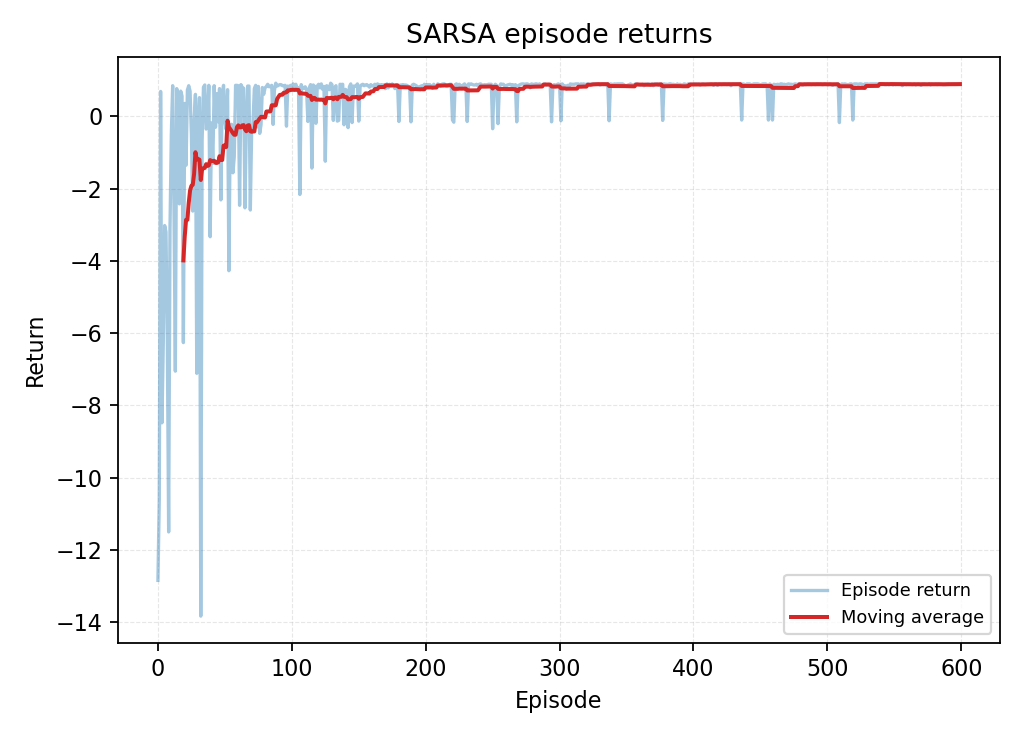
\includegraphics[width=0.8\linewidth]{sarsa_returns.png}
  \caption{SARSA 回报曲线,展示 \(\varepsilon\)-贪心策略下的收敛趋势}
  \label{fig:sarsa_returns_cn}
\end{figure}

\begin{figure}[H]
  \centering
  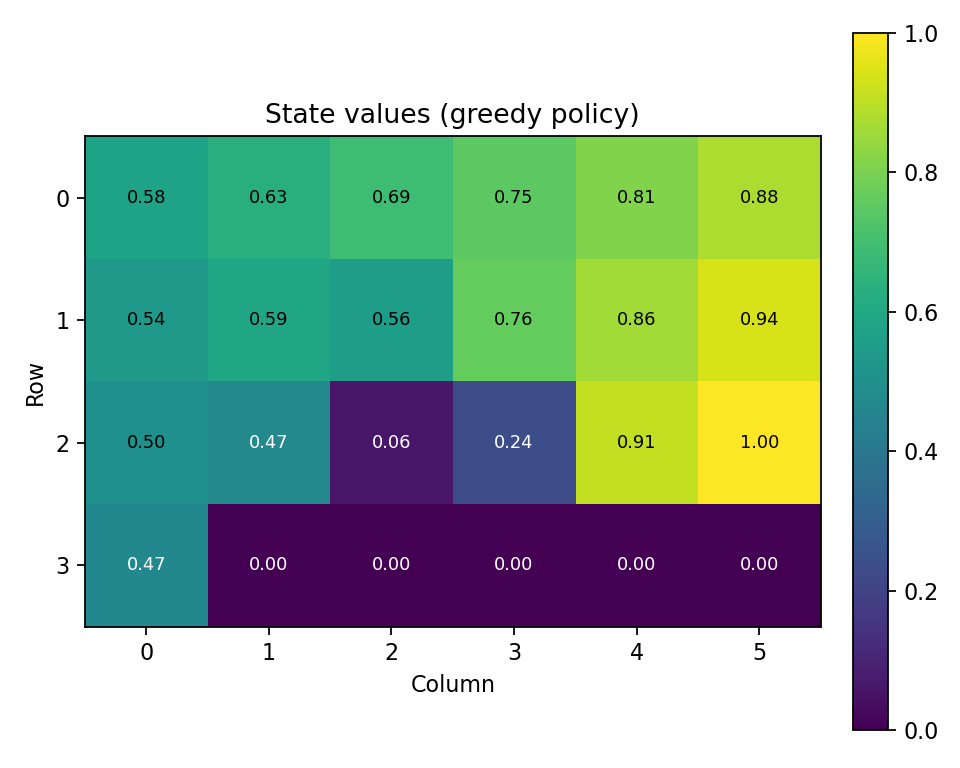
\includegraphics[width=0.82\linewidth]{sarsa_state_values.png}
  \caption{最终状态价值热力图,体现算法在危险区域的保守策略}
  \label{fig:sarsa_state_values_cn}
\end{figure}

\FloatBarrier
\section{总结}
SARSA 将探索行为纳入更新目标,适合风险敏感的强化学习任务。通过调节学习率与探索策略,可实现稳定收敛。示例演示了回报随训练稳定提升,以及学习到的价值函数如何回避“悬崖”区域。

\end{document}